\documentclass[12pt]{article}
\usepackage[utf8]{inputenc}
\usepackage[english]{babel}
\usepackage{amsmath}
\usepackage{amsfonts}
\usepackage{amssymb}

\usepackage[pdftex]{graphicx}
\usepackage{epsfig}
\usepackage{epstopdf}
\usepackage{multirow}

\usepackage{rotating}

%% MATH -----------------------------------------------------------
\newcommand{\modulo}[1]{\vert#1\vert}
\newcommand{\norm}[1]{\left\Vert#1\right\Vert}
\newcommand{\abs}[1]{\left\vert#1\right\vert}
\newcommand{\set}[1]{\left\{#1\right\}}
\newcommand{\Real}{\mathbb R}
\newcommand{\eps}{\varepsilon}
\newcommand{\To}{\longrightarrow}
\newcommand{\BX}{\mathbf{B}(X)}
\newcommand{\A}{\mathcal{A}}
\newcommand{\Cero}{\mathbf 0}


%% DATOS AUTORES --------------------------------------------------
\author{Pedro Diamel Marrero Fernandez \\ Juan González Hidalgo} 
\title{Projeto AM 2016-1: MVFCMddV and Multiclasification}

\begin{document}

\maketitle

%\begin{abstract}
%\end{abstract}


\section*{Introduction}
Uma das áreas actualmente mais desenvolvidas do mundo da inteligência artificial é a Aprendizagem de Máquina, na qual se desenvolvem diferentes algoritmos e técnias que permitem aprender ao computador para seu desenvolvimento em diferentes tarefas.Neste abordagem os algoritmos de agrupamento desempenham um papel fundamental. O objetivo deste trabalho é a implementação e avaliação do método de clusters MVFCMddV( Multi-view relacional fuzzy c-medoids vectors clustering algorithm), assim como a combinação dos classificadores para a classificação de dados utilizando várias funcionalidades(feauters supspaces).

\section{Methods}
En este punto se realiza una breve descripcion de los metodos y algoritmos empleados en este trabajo. 

\subsection{MVFCMddV Algoritm}

\subsection{Bayes}
O Teorema de Bayes é usado para calcular a probabilidade a posteriori de um evento, dados sua probabilidade a priori e a verossimilhança do novo dado. A descrição anterior é determinada pela seguinte equação:
\begin{equation}
\mathbf{P(w_j\vert x)= \dfrac{p(x\vert w_j) P(w_j)}{p(x)} }
\end{equation}
onde $\mathbf{P(w_j\vert x)}$ é a probabilidade a posteriori, a verossimilhança  é dada pela casse $\mathbf{w_j}$ cujo $\mathbf{p(x\vert w_j)}$ é o maior é mais verossímil de ser a verdadeira classe. E a evidência $\mathbf{p(x)}$ determinada pela equação $\mathbf{\Sigma_{j=1}^{n} p(x\vert w_j) P(w_j)}$ é o fator de escala que garante que a
soma das probabilidades a posteriori é 1.
\subsection{MLP}
Para resolver problemas não linearmente separáveis e de classificação utilizando Redes Neurais Artificias, a alternativa mais utilizada é adicionar uma o mais camadas intermediárias ou escondidas. As redes do tipo perceptron multicamadas $\textbf{(MLP)}$ apresentam uma ou mais camadas intermediárias de neurônios e uma camada de saída. Elas são treinadas com um algoritmo de retropropagação do erro(Back Propagation).
O modelo é arranjado em 3 camadas na figura \ref{fig:mlp}.


\begin{figure}[h]
\centering
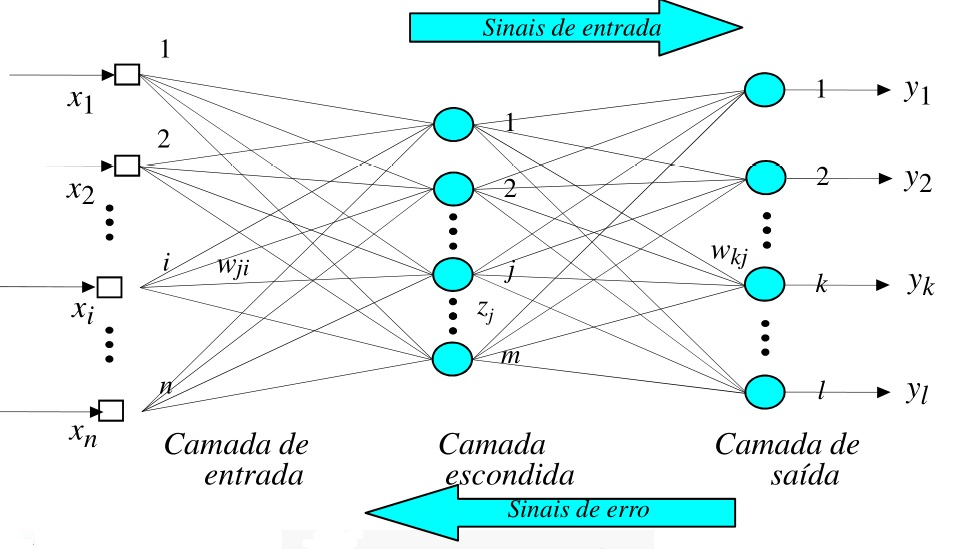
\includegraphics[width=4.5in]{../out/mlp.jpg}
\caption{Red Neural do tipo MLP}
\label{fig:mlp}
\end{figure} 

Estas redes de tipo $\textbf{MLP-BP}$ tem um alto poder de representação, larga aplicabilidade, facilidade de implementar a aprendizagem e uma boa capacidade de generalização. Mas também tem seu aprendizagem de transformações complexas pode demorar para convergir, possuem limitações decorrentes do gradiente descendente e a generalização não e garantida(problema de sobretreinamento).
\subsection{SVM}
As máquinas de vetores de suporte(support vector machines - $\textbf{SVMs}$ ) vêm recebendo crescente atenção da comunidade de Aprendizagem de Máquina nos últimos anos. Elas tem como características principais:
\begin{itemize}
    \item Capacidade de generalização alta, evitando sobretreinamento.
    \item Robustez para categorização de dados com dimensões altas, que tendem a ser sobretreinados em outros classificadores pois muitas micro-características são pouco discriminantes.
    \item Convexidade da função objetivo pois esta é uma função quadrática com apenas um ótimo global. 
    \item Teoria bem estabelecida nas áreas de matemática e estatística.
\end{itemize}


\subsection{Multiclasification sistem}


\begin{figure}[h]
\centering
\includegraphics[width=4.5in]{../out/system-multclassy.eps}
\caption{Arquetetura de systema multiclasificadores emplegadas.}
\label{fig:mult_system_classy}
\end{figure}  



\section{Result and Discussion }


\subsection{MVFCMddV methods evaluate in synthetics data.}

Para la generacion de los datos sinteticos se empleo un generador aleatorio para datos normales multivarios y se generaron tres muestras de parametros: 

$$\mu_1 = [2, 2], \ \mu_2 = [-2, -1], \ \mu_3 = [7, -1] $$
$$\Sigma_1 = \left[ \begin{matrix}
2 & 0 \\ 
0 & 1
\end{matrix} \right], 
\Sigma_2 = \left[ \begin{matrix}
1 & 0 \\ 
0 & 1
\end{matrix} \right], 
\Sigma_2 = \left[ \begin{matrix}
1 & 0 \\ 
2 & 0
\end{matrix} \right] $$

Para generar tres señales diferentes a partir de una de ellas fueron rotados los datos en $\theta = 30$ y $\theta = 90$ grados ($X_i = R_i(\theta)*X$). Los resultados obtenidos para las tres señales se muestran en la Fig. \ref{fig:xy_sinteticos}.

\begin{figure}[h]
\centering
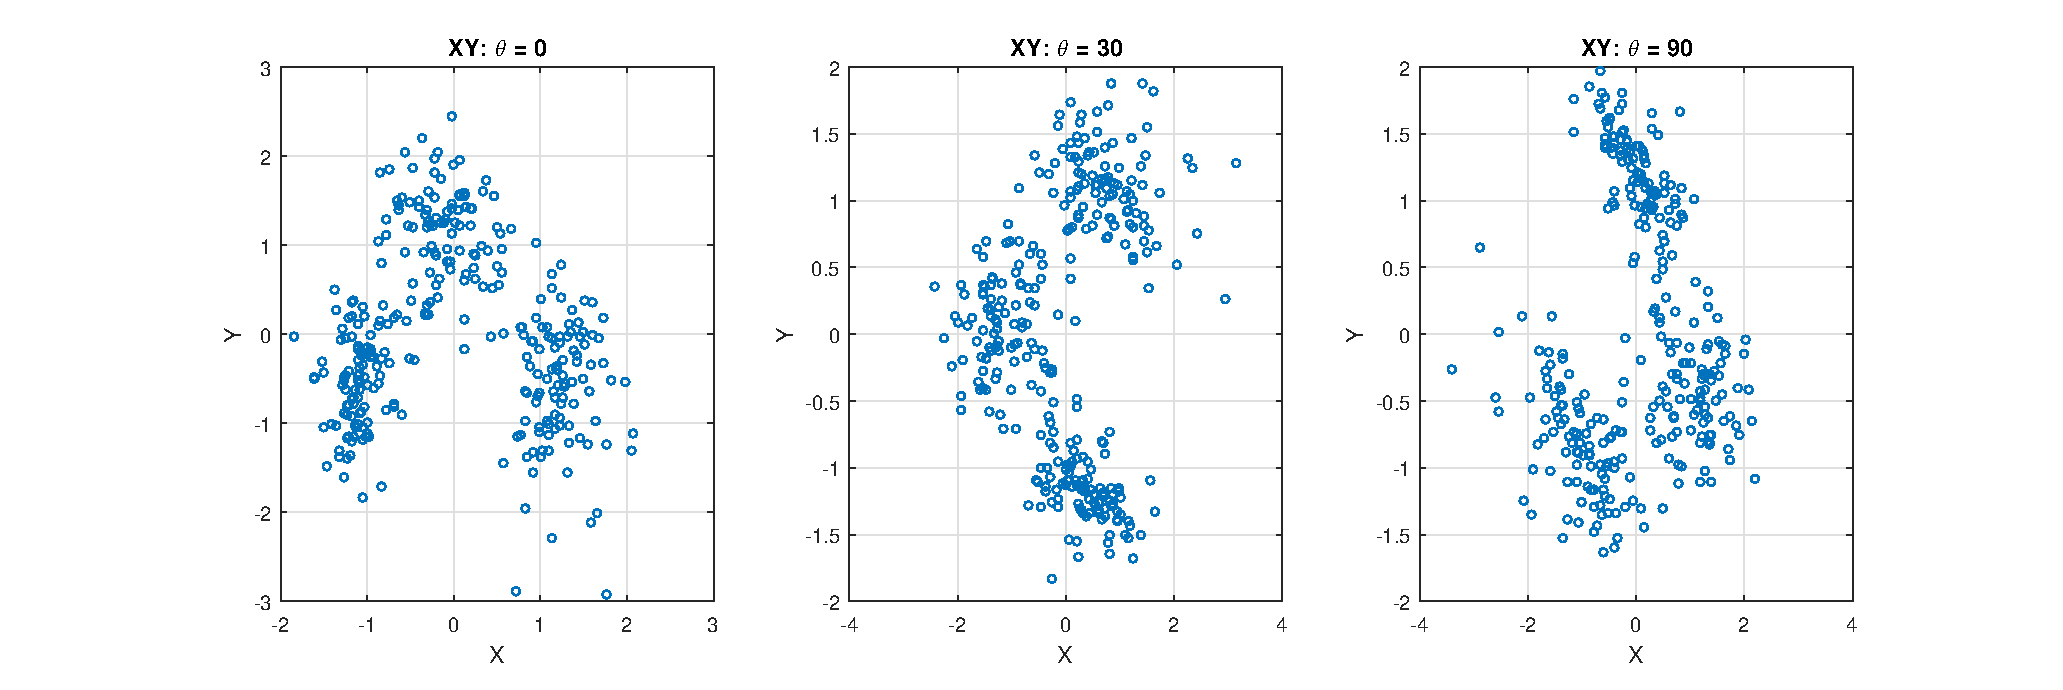
\includegraphics[width=4.5in]{../out/xy-sinteticos.eps}
\caption{Datos sinteticos generados.}
\label{fig:xy_sinteticos}
\end{figure}  

Para la aplicacio del metodo MVFCMddV se empleo la siguiente configuracion, $K = 3$, $m = 1.2$, $T = 10$, $\epsilon = 1e^{-500}$. La Fig. \ref{fig:cluster_datos_sinteticos} muestra los resultados optenidos. En este caso se obtuvo un corrected Rand index (CR) de $0.98$.


\begin{figure}[h]
\centering
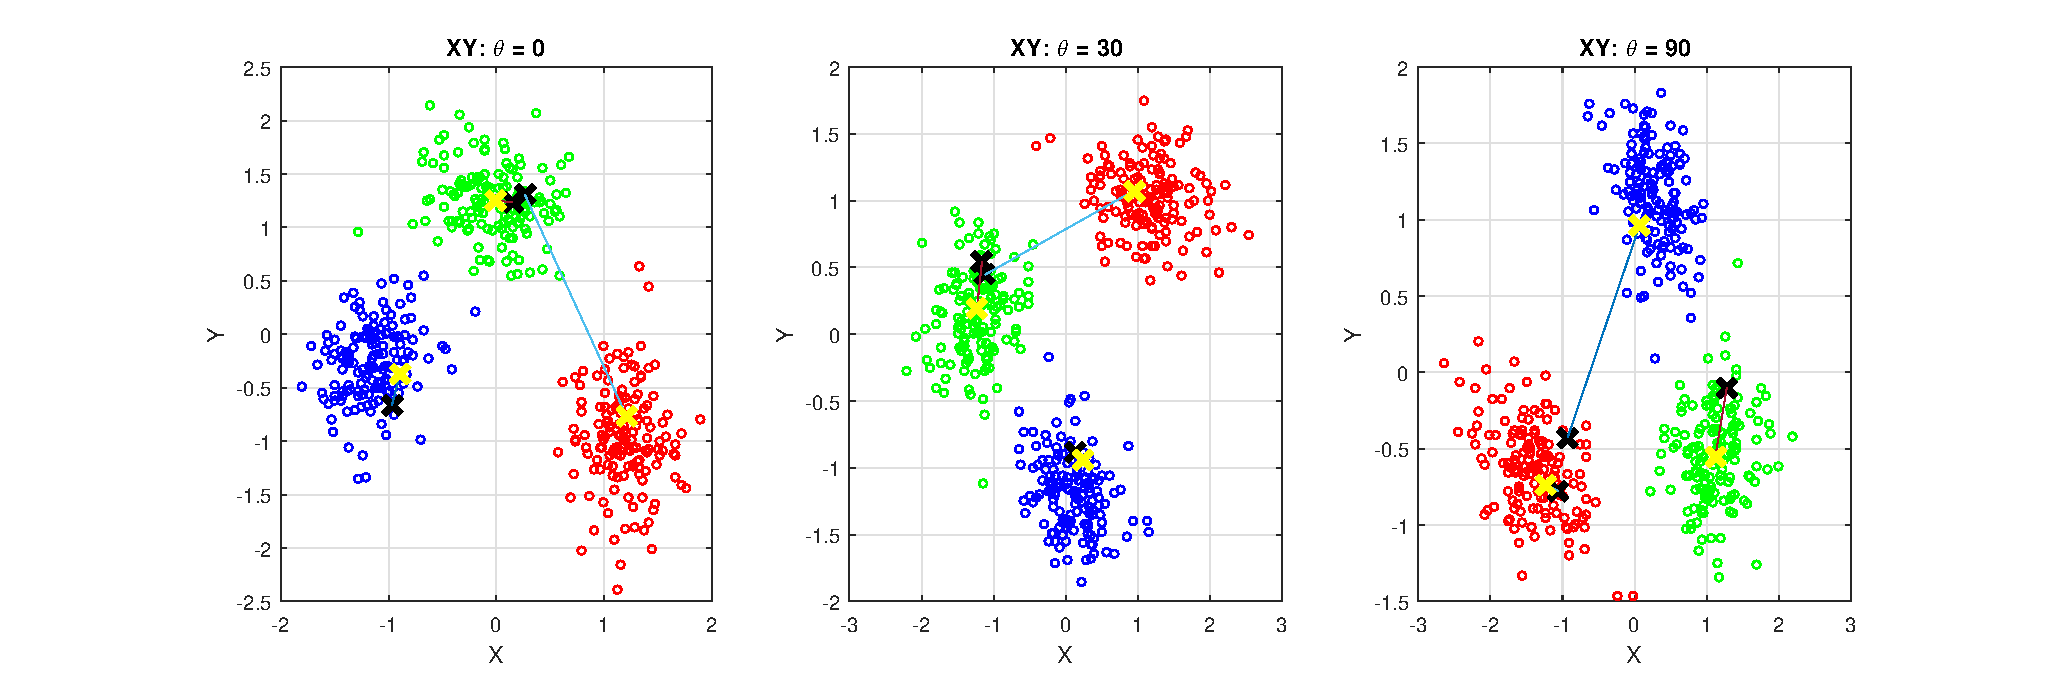
\includegraphics[width=4.5in]{../out/clusters-gauss-3.eps}
\caption{Resultados optenidos por MVFCMddV. En negro se muestran los centroides iniciales y en amarillo los centroides finales optenidos por el sistema.}
\label{fig:cluster_datos_sinteticos}
\end{figure}  


\subsection{MVFCMddV methods evaluate in real data.}

Para evaluar el metodo  MVFCMddV con datos reales fue empleada Multiple Features Data Set[XXX]. This dataset consists of features of handwritten numerals (`0'--`9') extracted from a collection of Dutch utility maps.

\begin{figure}[h]
\centering
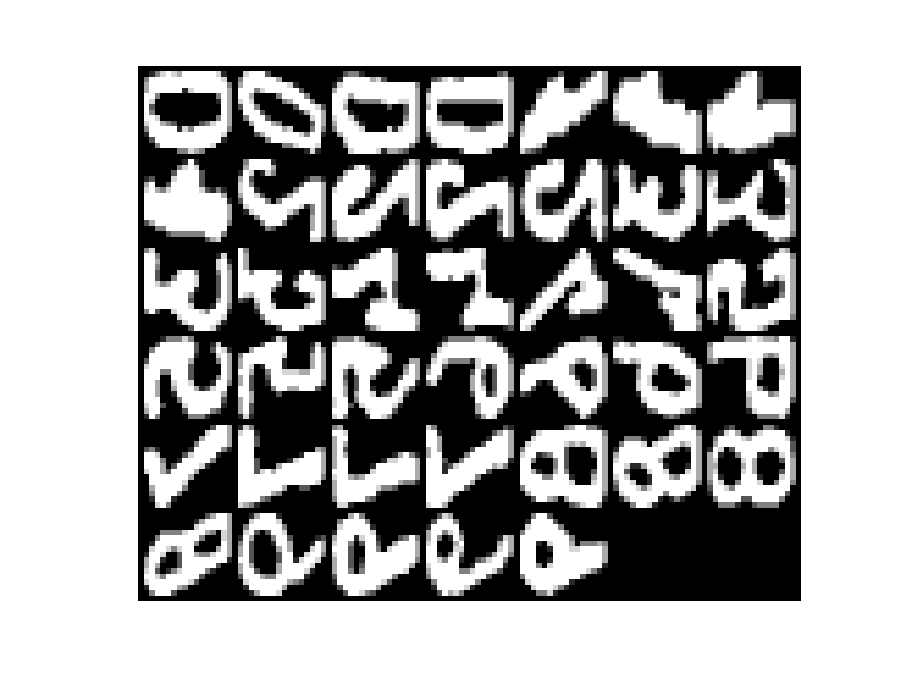
\includegraphics[width=3.5in]{../out/data-base.eps}
\caption{Multiple Features Data Set.}
\label{fig:data_base}
\end{figure}  

This dataset consists of features of handwritten numerals (`0'--`9') extracted from a collection of Dutch utility maps. 200 patterns per class (for a total of 2,000 patterns) have been digitized in binary images. These digits are represented in terms of the following six feature sets (files): (1) mfeat-fou: 76 Fourier coefficients of the character shapes; (2) mfeat-fac (FAC): 216 profile correlations; (3) mfeat-kar (KAR): 64 Karhunen-Love coefficients; (4) mfeat-pix (PIX): 240 pixel averages in $2 \times 3$ windows; (5) mfeat-zer (ZER): 47 Zernike moments; (6) mfeat-mor (MOR): 6 morphological features. In each file the 2000 patterns are stored in ASCI on 2000 lines. The first 200 patterns are of class `0', followed by sets of 200 patterns for each of the classes `1' - `9'. Corresponding patterns in different feature sets (files) correspond to the same original character. The source image dataset is lost. Using the PIX dataset sampled versions of the original images may be obtained ($15 \times 16$ pixels).

Se selecciono para hacer los experimentos los subespacios de caracteristicas determinados por FOU, KAR y ZER. Fue executado 100 veses o algoritmo MVFCMddV simultaneamente para las 3 matrizes de dissimilaridade correspondientes a cada subspacio. En este caso se empleo la siguiente configuracion: $K =10$, $m = 1.6$, $T = 150$, $\epsilon = 1e^{10}$.

En este caso se obtuvo un CR index de $0.108$ y un F-mesure de $0.345$. 




\subsection{MVFCMddV methods in compress image problems.}

In a straightforward 24-bit color representation of an image, each pixel is represented as three 8-bit unsigned integers (ranging from 0 to 255) that specify the red, green and blue intensity values. This encoding is often refered to as the RGB encoding. Existen otros espacios de representacion del color como el CIELAB, HSB CMYK. El objetivo de este esperimento es valorar la reducion del numero de colores en el espacio RGB empleando ademas el espacio CIELAB. Una hipotesis valida es que la informacion de este nuevo espacio puede cotribuir a la creacion de clusters mas conveniente en este tipo de problemas.  

Como se puede obsevar en la Fig. \ref{fig:image_compress} se obtiene una buena aproximacion de la imagen original. Esta nueva imagen puede ser representada como 4-bits por pixel mas un diccionario de $16\times24$. The original image required 24 bits for each one of the $64X64$ pixel locations, resulting in total size of $64\times64\times24 = 98.304$ bits. The new representation requires some overhead storage in form of a dictionary of 16 colors, each of which require 24 bits, but the image itself then only requires 4 bits per pixel location. The final number of bits used is therefore $16\times24 + 64\times64\times4 = 16.384$ bits, which corresponds to compressing the original image by about a factor of 6.


\begin{figure}[h]
\centering
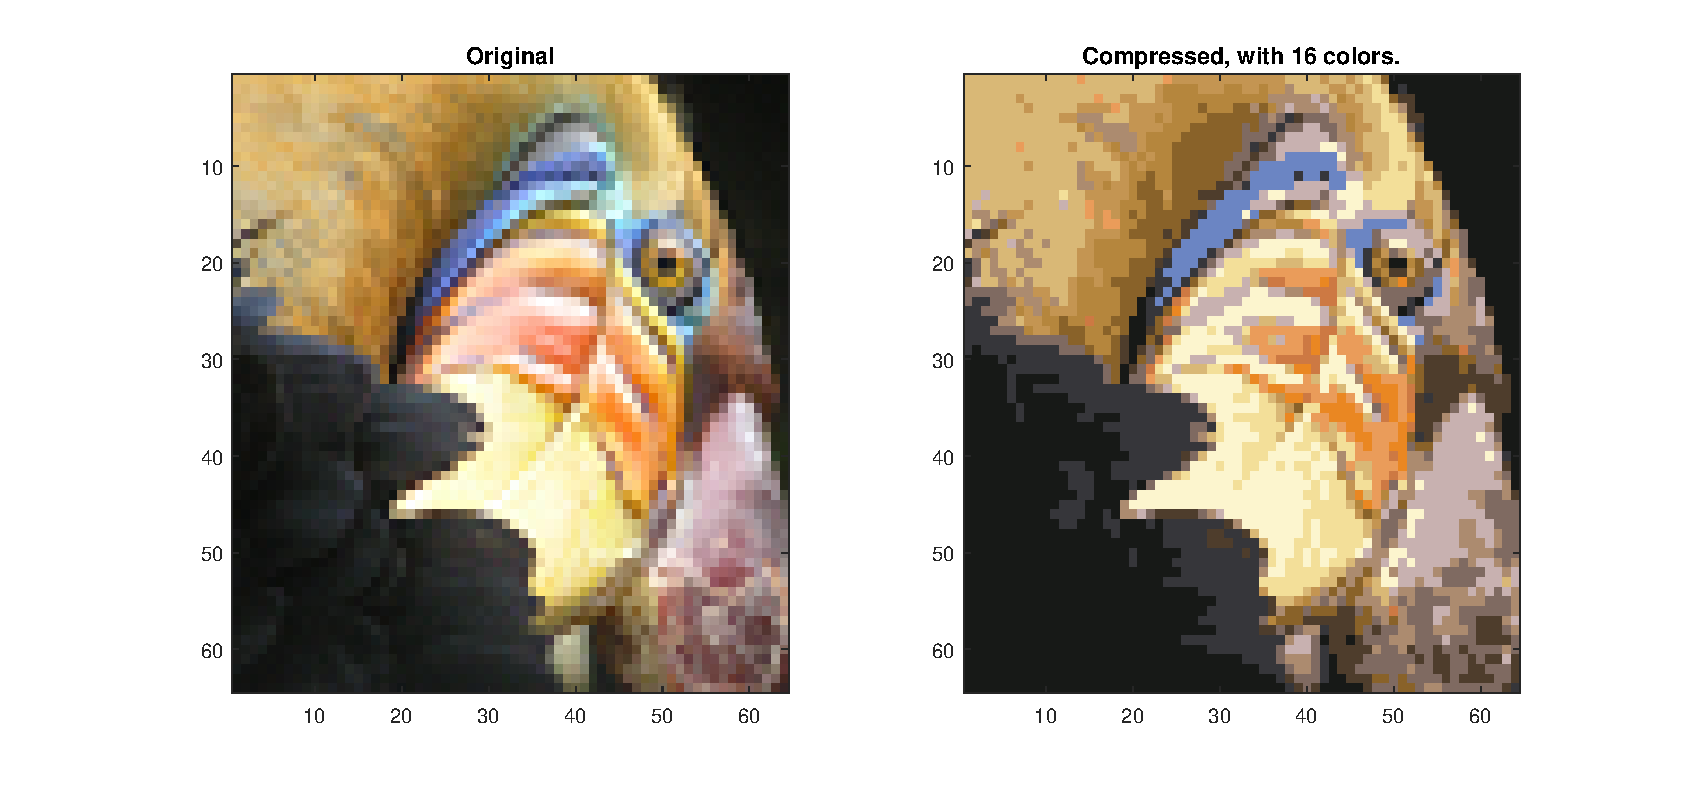
\includegraphics[width=5.5in]{../out/image-compress-16.eps}
\caption{Original and reconstructed image (when using MVFCMddV to compress the image).}
\label{fig:image_compress}
\end{figure}  


\subsection{Multiclasifcador system for multiples signal}

En este caso tambien fue empleada la base de datos Multiple Features Data Set. Se empleo 40-kfold cross validation, empleando conjunto de validacion para ajustar los paramentros de los metodos SVM y MLP. En el caso de SVM se ajusto el parametro de regularizacion $C$ e igualmente en el MLP se ajusto el parametro de regularizacion $\lambda$. La Fig. \ref{fig:roc_curve} muestra las curvas ROC corespondiente al primer fold para el ajuste de los parametros. Como se puede observar la señal KAR es la señal que mas explica cada una de las clases. 


\begin{figure}[!h]
\centering
\begin{tabular}{cc}
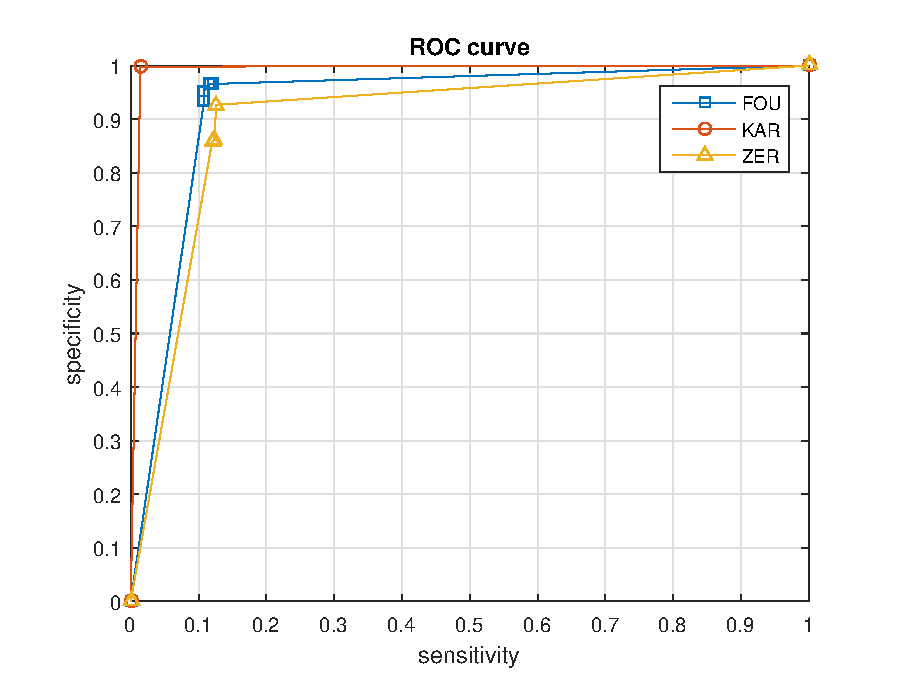
\includegraphics[width=2.5in]{../out/svm-roc.eps}&
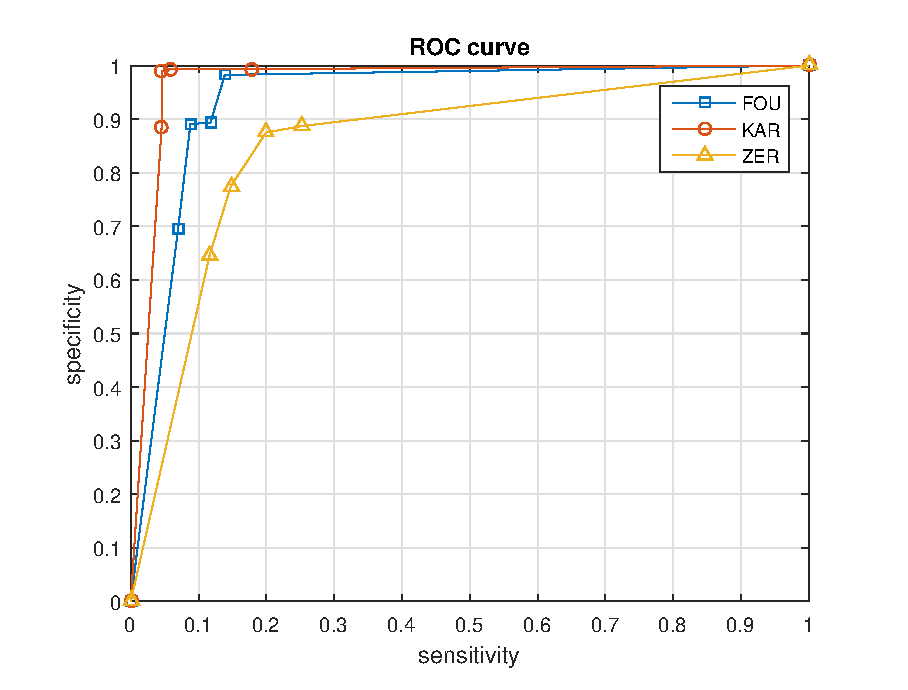
\includegraphics[width=2.5in]{../out/mlp-roc.eps} \\
a) SVM  & b) MLP
\end{tabular}
\caption{ROC curve. variando el termino de regularizacion en cada caso.}
\label{fig:roc_curve}
\end{figure}
 
 
%% Analidis estadistico de los resultados...
%% Analisis de los datos
 
La tabla \ref{tab:analisis_data} muestra un resumen de los resultads obtenidos en cada uno de los algoritmos empleado de manera individual vs la combinacion de todos (COMB) empleando voto mayoritario (VM). Los mejores resultados fueron obtenidos emplando , MLP y COMB con voto mayoritario con un $0.92 \pm 0.03$. Todos los metodo obtuvieron para un juego de datos un 0.98 como maximo valor y el enfoque bayesiano obtuvo el peor valor en una de las iteraciones.
 
%% R
%%        B              SVM              MLP             ALL        
%% Min.   :0.800   Min.   :0.8600   Min.   :0.860   Min.   :0.8600  
%% 1st Qu.:0.880   1st Qu.:0.9000   1st Qu.:0.895   1st Qu.:0.9000  
%% Median :0.900   Median :0.9200   Median :0.920   Median :0.9200  
%% Mean   :0.901   Mean   :0.9195   Mean   :0.915   Mean   :0.9255  
%% 3rd Qu.:0.920   3rd Qu.:0.9400   3rd Qu.:0.940   3rd Qu.:0.9600  
%% Max.   :0.980   Max.   :0.9800   Max.   :0.980   Max.   :0.9800  
%%> sd(DB$B)
%%[1] 0.037
%%> sd(DB$SVM)
%%[1] 0.035
%%> sd(DB$MLP)
%%[1] 0.032
%%> sd(DB$ALL)
%%[1] 0.034
 
 
\begin{table}[!h]
\renewcommand{\arraystretch}{1.3}
\caption{Sumario de los Resultados Obtenidos. }
\label{tab:analisis_data}
\centering
\begin{tabular}{c}
\begin{tabular}{rcccc}
\hline
         &B   &     SVM  &  MLP   &  COMB     \\
\hline     
 Min.    &0.800   &0.860   &0.860   &0.860\\  
 1st Qu. &0.880   &0.900   &0.895   &0.900\\  
 Median  &0.900   &\textbf{0.920}   &\textbf{0.920}   &\textbf{0.920}\\  
 Sd      &0.037   &0.035   &0.032   &0.034\\
 Mean    &0.901   &0.920   &0.915   &0.926\\  
 3rd Qu. &0.920   &0.940   &0.940   &0.960\\  
 Max.    &0.980   &0.980   &0.980   &0.980\\  
\hline 
\end{tabular}\\
\multicolumn{1}{p{2.8in}}{ B: Classificador bayesiano, SVM: Super vector machine, MLP: multilayer perceptron, COMB: Regla de combinacion por voto mayoritario. }
\end{tabular}
\end{table} 
 
Como se puede observar en la Fig. \ref{fig:densidade_acc} los resultados obtenidos son bien similares y en la mayoria de los casos con una tendencia a la normalidad fundamentalmente en el caso del modelo bayesiano y el MLP. No obstante en el caso de la salida de COMB y SVM no parece tener distribucion normal. 

\begin{figure}[h]
\centering
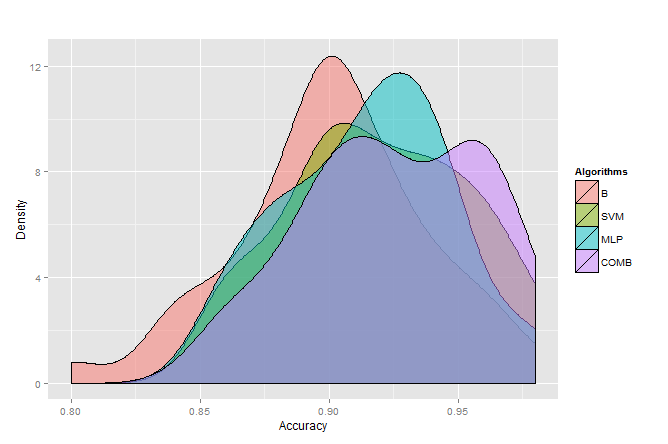
\includegraphics[width=4.5in]{../out/density-graph.png}
\caption{Grafico de densidade de las muestras correspondientes a la salida de error de cada metodo testado.}
\label{fig:densidade_acc}
\end{figure} 

En la Fig. \ref{fig:boxplot_acc} muestra que el metodo COMB no es simetrico, no obstante este metodo presenta mayor volumen de informacion entre el segundo y tercer quartil. Igualmente este grafico nos permite observar que el comportamiento de los metodos es muy similar. En el caso del modelo Bayesiano el mismo presenta un outliner, lo que indica que en al menos un iteracion do kfold este obtuvo resutados por debajo de 0.85. 

\begin{figure}[!h]
\centering
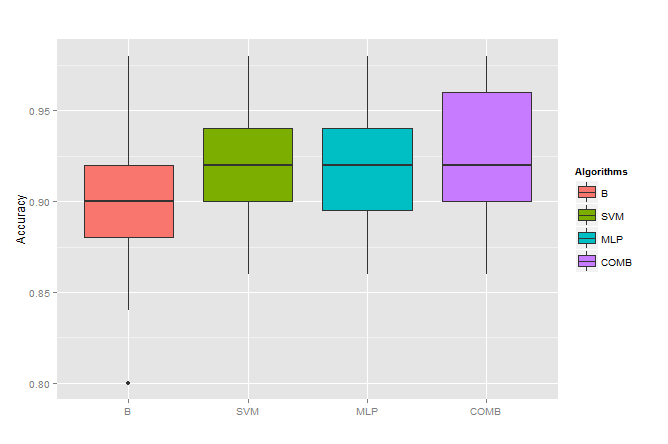
\includegraphics[width=4.5in]{../out/boxplot-errors.png}
\caption{Box plot de los metodos evaluados.}
\label{fig:boxplot_acc}
\end{figure}  


%% Test de aderencia

Para validar el supuesto de que los resultados no siguen una distribucion normal se aplico el test de aderencia  Lilliefors test (Kolmogorov-Smirnov para o caso de normalidad). Este test se aplica bajo la hipotesis nula de que los datos siguen una distribucionn normal. El p valor obtenido para el caso COMB, por ejemplo, fue de 0.006, lo cual rechaza la hipotesis nula con una cofianza de 0.5. Por tanto podemos concluir que la salida de alguno de los metodos, no presentan distribucion normal. De aqui que el posterior analises sea realizado a traves de métodos no parametricos. 

%%R
%%Lilliefors (Kolmogorov-Smirnov) normality test
%%data:  X
%%D = 0.16642, p-value = 0.006916

%% Prueba de hipotesis entre los clasificadores
Para la comparacion de los metodos fue aplicado un test de hipotesis para muestras pareadas. En particular en este caso empleamos la variante no parametrica Analysis of Variance (ANOVA) para dos factores, Friedman-test, bajo las siguientes hipotesis:

\begin{alignat*}{2}
  H_0:  & \ M_1 = M_2 = ... =M_n \\
  H_1:  & \ \exists M_i,M_j \ | \ M_i\neq M_j
\end{alignat*}

Para este experimento se obtuvo un p valor de 0.0002, lo cual rechaza la hipotesis nula de que las medianas de los metodos testados son iguales, con una significacioa de 0.05. Para determinar cuales metodos presentan diferncias significativas entre ellos fue aplicado el post test de Nemenyi. 

La tabla \ref{tab:test_nemeyi} muestra los resultados alcanzados para el p-valor dos a dos. Como se puede observar el modelo bayesiano presenta diferencias significativas con respecto a los demas metodos. Los metodos SVM, MLP y la combinacion COMB, no presentan diferencias significativas. 

\begin{table}[!h]
\renewcommand{\arraystretch}{1.3}
\caption{Nemenyi Multiple Comparison Test. }
\label{tab:test_nemeyi}
\centering
\begin{tabular}{c}
\begin{tabular}{rccc}
\hline
    &B       &SVM     &MLP         \\    
\hline                             
SVM &0.06497 &-       &-           \\  
MLP &0.07245 &0.99997 &-           \\
COMB &0.00047 &0.45437 &0.42808    \\
\hline 
\end{tabular}\\
\multicolumn{1}{p{2.8in}}{ B: Classificador bayesiano, SVM: Super vector machine, MLP: multilayer perceptron, COMB: Regla de combinacion por voto mayoritario. }
\end{tabular}
\end{table}

De manera general los metodos SVM, MLP y COMB, persentan resultados semejantes. En el caso de COMB precisa un costo computacional proporcional a la cantidad de modelos que se emplean. Se concluye que el amento de rendimiento proporsionado por COMB no justifica su empleo para estas condiciones, se recomienda el uso de el metodo SVM o MLP. 


%%%Matlab
%%%Result: 
%%%E:7.450000e-02 St: 3.448894e-02 
%%%Friedman test 
%%%Rejeita H_0 com um nivel de 2.226e-04 
%%%Nemenyi pos-hoc: 
%%%Matrix p: 
%%%    1.0000    0.0815    0.0919    0.0005
%%%    0.0815    1.0000    1.0000    0.8457
%%%    0.0919    1.0000    1.0000    0.7778
%%%    0.0005    0.8457    0.7778    1.0000
%%%
%%%Matrix H: 
%%%     0     0     0     1
%%%     0     0     0     0
%%%     0     0     0     0
%%%     1     0     0     0
%%%
%%%Bonferroni pos-hoc: 
%%%Matrix p: 
%%%    0.0001
%%%    0.2114
%%%    0.1945
%%%    1.0000
%%%
%%%Matrix H: 
%%%     1
%%%     0
%%%     0
%%%     0


%%% R
%Friedman rank sum test
%
%data:  X
%Friedman chi-squared = 19.432, df = 3, p-value = 0.0002226
%
%> test_friedman$ptnemenyi
%
%	Pairwise comparisons using Nemenyi multiple comparison test	
%             with q approximation for unreplicated blocked data 
%
%data:  X 
%
%    B       SVM     MLP    
%SVM 0.06497 -       -      
%MLP 0.07245 0.99997 -      
%ALL 0.00047 0.45437 0.42808
%
%P value adjustment method: none 




\end{document}